\documentclass[conf]{new-aiaa}
%\documentclass[journal]{new-aiaa} %for journal papers
\usepackage[utf8]{inputenc}


\usepackage{graphicx}
\usepackage{amsmath}
\usepackage[version=4]{mhchem}
\usepackage{siunitx}
\usepackage{longtable,tabularx}
\setlength\LTleft{0pt} 
\usepackage{subfig}
% Keywords command
\providecommand{\keywords}[1]
{
  \small	
  \textbf{\textit{Keywords---}} #1
}
\hypersetup{colorlinks=true, urlcolor=blue, linkcolor=black, citecolor=black}

\title{Multifidelity aeroelastic optimization with application to a BWB}

\author{Gilberto Ruiz Jiménez\footnote{Insert Job Title, Department Name, Address/Mail Stop, and AIAA Member Grade (if any) for first author.} and Joan Mas Colomer\footnote{Insert Job Title, Department Name, Address/Mail Stop, and AIAA Member Grade (if any) for second author.}}
\affil{Université de Toulouse, Toulouse, France, 31400}
\author{Joseph Morlier\footnote{Insert Job Title, Department Name, Address/Mail Stop, and AIAA Member Grade (if any) for third author.}}
\affil{Université de Toulouse, Toulouse, France, 31400}

\begin{document}
\twocolumn[
\begin{@twocolumnfalse}
\maketitle

\begin{abstract}
A multifidelity approach for the solution of aeroelastic optimization problems is developed using open-source tools. The Multidisciplinary Optimization problem is managed via OpenMDAO and a dedicated python library. Aerodynamics are solved with PANAIR, with a detailed mesh for the High-Fidelity case and a coarser mesh for the Low-Fidelity one. Structural displacements are computed via NASTRAN and transferred to the aerodynamic mesh with radial basis functions (RBF). The program starts solving the coupled problem at a low fidelity level, and once some predefined convergence tolerance is reached, the high fidelity solver is called. The Multidisciplinary Analysis (MDA) solution is then treated by the outer-loop optimizer, which modifies the geometry in order to comply with design constraints and minimize fuel consumption. The method was implemented on the NASA CRM wing section, on a Blended Wing Boyd (BWB) concept, and using analytical test functions. It was found that a simple transfer of the displacement field between fidelities helps to slightly reduce optimization iterations while improving constraint convergence. 
\end{abstract}
\keywords{Multifidelity, aeroelasticity, BWB, MDO}
\newline
\newline

\end{@twocolumnfalse}
]
\footnotetext[1]{M.Sc. Student, ISAE-SUPAERO, 10 Av. Edouard Belin, 31400, Toulouse, France, gilberto.ruiz-jimenez@student.isae-supaero.fr}
\footnotetext[2]{Postdoctoral Researcher, DMSM, 10 Av. Edouard Belin, 31400, Toulouse, France, joan.mas-colomer2@isae-supaero.fr}
\footnotetext[3]{Professor, Institut Clément Ader (ICA), CNRS, ISAE-SUPAERO, UPS, INSA, Mines-Albi, 3 rue Caroline Aigle, 31400 Toulouse, France, Joseph.morlier@isae-supaero.fr, AIAA Member}
%\section{Nomenclature}

%Uncomment nomenclature table if needed
%{\renewcommand\arraystretch{1.0}
%\noindent\begin{longtable*}{@{}l @{\quad=\quad} l@{}}
%$MDO$ & MultiDisciplinary Optimization \\
%$MDA$ & MultiDisciplinary Analysis \\
%$MDF$ & MultiDisciplinary Feasible \\
%$BWB$ & Blended Wing Body \\
%$TRMM$ & Trust Region Model Management \\
%$MLE$ & Maximum Likelihood Estimate \\
%$RANS$ & Reynolds-Averaged Navier–Stokes equations \\
%$IDF$ & Individual Discipline Feasible \\
%$COBYLA$ & Constrained Optimization By Linear Approximation \\
%$RBF$ & Radial Basis Functions 
%\end{longtable*}}

\section{Introduction}
\lettrine{M}{odern} engineering design problems rely increasingly on the interdisciplinary interactions between subsystems. As a consequence, multidisciplinary design strategies have been developed, these allow to manipulate design variables from various disciplines simultaneously. Moreover, the incorporation of optimization tools within these methodologies leads to what is referred collectively as Multidisciplinary Design Optimization (MDO).    
The present work deals with the interaction of aerodynamics and structures (so called Fluid-Structure Interaction, FSI), which is a key feature in aircraft design. Coupled aeroelastic analyses allow a better prediction of the aerodynamic forces and structural displacements that the aircraft experiences in real flight, hence, an MDO platform is implemented in order to study these interactions. \par 
Each discipline inside the MDO problem requires a solver that computes its effects on the global problem, with the aerodynamic solution being the main source of computational cost. High fidelity CFD analyses offer accurate results, but at the expense of high computational time. On the other hand, potential flow theory, and its computational implementation, the panel codes, offer reasonable approximations with low computational demands. The main goal of this project is to efficiently use low-fidelity analyses, combined to high-fidelity ones, to conduct aeroelastic optimizations, with an application to a Blended Wing Body (BWB) configuration. \par
The starting point for the bibliography research is a Survey of Multifidelity Methods by Peherstorfer \cite{peherstorfer2018survey}, where a variety of alternatives are listed and classified. Surrogate modelling is a global optimization strategy. It uses co-kriging as a regression technique in order to link High-Fidelity sources with one or many Low-Fidelity functions. This correlated model can be used to find optimal solutions faster \cite{Forrester2007}. On the other hand, simpler approaches such as a linear regression are found to offer a good balance between accuracy, cost and simplicity \cite{Zhang2019}. Other advantages include: ease to combine many low-fidelity sources and robustness for High-Fidelity samples with the presence of noise \cite{Zhang2019}. \par 
Newton methods and their variations have been explored as well. Jovanov and Breuker propose to solve the High-Fidelity problem by adding an aerodynamic correction load to the solution of the Low-Fidelity equation. The defect-correction method accelerates the convergence compared to the Quasi-Newton method \cite{Jovanov2015}. This last case does not consider the methods as black-boxes, but rather exploits the fact that the algorithms of both fidelity levels are known and can be modified at any stage to accommodate the necessary corrections between them. Scholz presents an Aggressive Space Mapping methodology, it solves for the low fidelity fluid–structure interaction solution and then feeds that information to a Quasi-Newton algorithm. The final results are obtained from a mapping function between both fidelity levels \cite{Scholcz2014}. \par
When it comes to the application of mutifidelity models to aerospace design, there are several publications on the subject. A Bayesian-enhanced Low-Fidelity correction proved the ability to maintain high-fidelity accuracy while reducing computational cost associated with the optimization of an airfoil shape \cite{fischer2018bayesian}. An aeroelastic optimization of a BWB was carried out by Bryson \cite{Bryson2019} using a new TRMM (Trust Region Model Management) approach. Its main difference is that it adds hybrid additive-multiplicative corrections (or bridge functions) to the low-fidelity analysis \cite{Bryson2019a}. Another approach to the aeroelastic optimization of a BWB is presented by Marques \cite{Marques2019}. The flutter boundary problem is solved with a contour location approach (i.e. the zero contour of the aeroelastic damping coefficient). It also incorporates an active learning strategy, where the model evaluations are selected iteratively based on how much they are estimated to improve the predictions. 
All of the aforementioned techniques require statistical processing and complex combinations of stochastic regression and surrogate functions. This work explored a simpler approach: transfering of information within the routines of the MDAO, taking advantage of the open-source tools at every step of the process. \par
%%%%DESCRIBIR LA ESTRUCTURA DEL ARTÍCULO%%%%%%%%
Section \ref{sec:methodology} describes in detail the proposed method, as well as the tools that were integrated in the MDAO and how they were programmed. Section \ref{sec:Demonstration} presents three different test approaches for the current formulation: optimizing the NASA Common Research Model (CRM) wing, optimizing a BWB configuration, and solving analytical optimization problems used to benchmark MDAO architectures. The results and perspectives for future work are discussed in section \ref{sec:conclusions}. 
\section{Methodology}
\label{sec:methodology}
A series of tools will be used together in order to create a complete multifidelity optimization solver. This section presents each of them as well as their coordinated implementation. 

\subsection{OpenMDAO}
First of all, the Multidisciplinary Design Analysis has to be established. The present work uses the OpenMDAO platform \cite{openmdao_2019}, an open source python library that allows the user to create, solve and optimize a wide variety of coupled problems. As a complement to this tool, the aerostructures package \cite{mascolomer:tel-02023612} assists the user in the creation of aerospace-related problems within the platform. \par The selected MDAO architecture is MultiDisciplinary Feasible or MDF, this means that the coupled problem is solved completely before the output is sent to the outer-loop optimizer. One of the advantages being that the optimization process can be interrupted before converging and the result at any point will satisfy consistency constraints (but not necessarily optimization constrains) \cite{gray2013standard}. There are many different MDAO architectures, in this case, the MDF was chosen because of the relatively simple problem (only 2 disciplines involved) and the ease of formulation. Another widely used architecture is Individual Discipline Feasible (IDF). It decouples the MDA, adding consistency constraints, and giving the optimizer control  of the coupling variables. This strategy generates a problem that is potentially much larger than MDF, depending on the number of coupling variables \cite{gray2013standard}. A wide study of different MDAO architectures is out of the scope of the current problem. \par
Figure \ref{fig:MDAOdiagram} shows a diagram of the MDAO formulation, the main components are the structural solver, the aerodynamic solver and a custom discipline called "Filter" that coordinates both fidelity levels. 


\begin{figure*}[htpb]
    \centering
    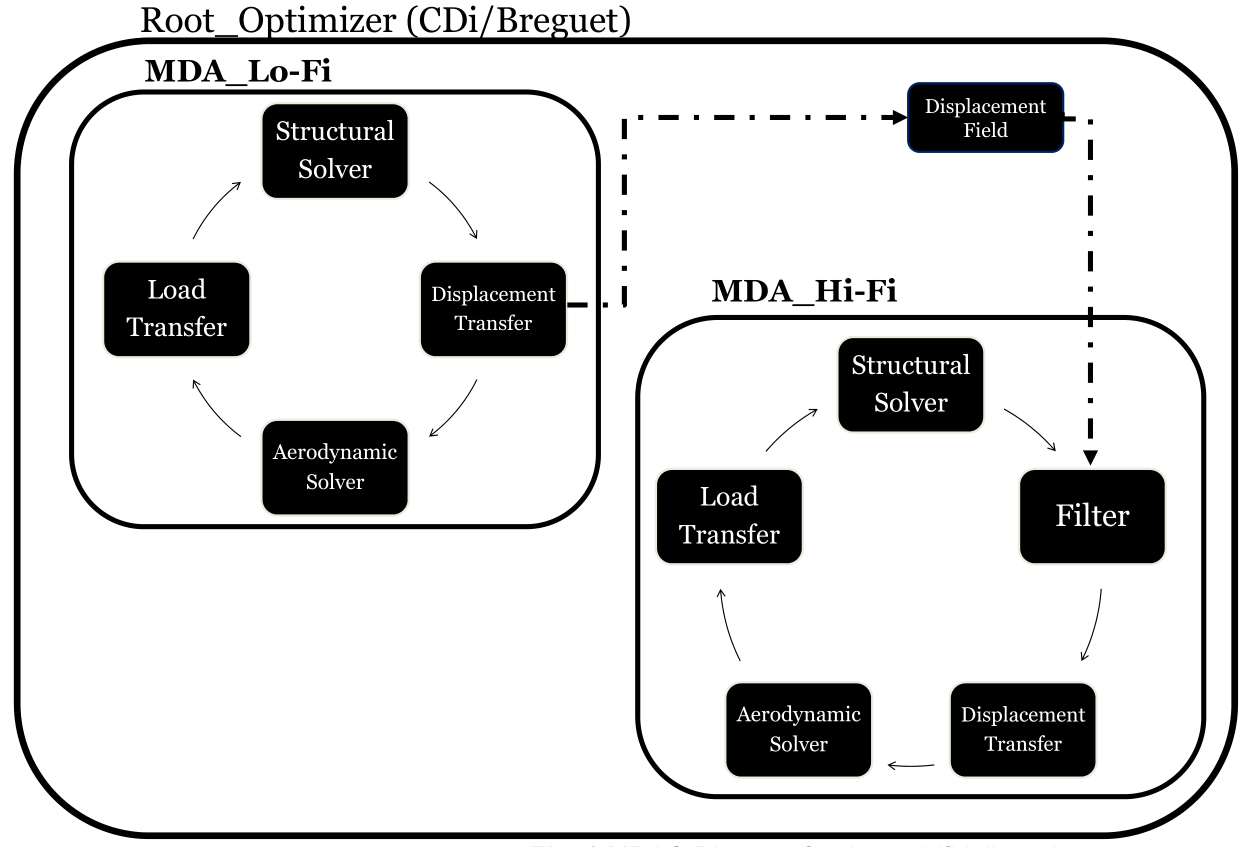
\includegraphics[width=0.75\textwidth]{images/MDAOdiagram.png}
    \caption{MDAO diagram of the coupled multifidelity problem}
    \label{fig:MDAOdiagram}
\end{figure*}


\subsection{Structural Solver}
NASTRAN simulations are treated using input files filled with instructions. These inputs are generated automatically at each run. Two files are needed to run the program, the first one, \verb|'nastran_static_template.inp'| looks mostly like a normal NASTRAN file but instead of the classical Nastran \verb|FORCE| cards, there are modified cards that include a dictionary key for each force component \cite{mascolomer:tel-02023612}, for example:
\begin{verbatim}
FORCE,201,33566,0,1.0,{Fx33566}, \\
{Fy33566},{Fz33566}
\end{verbatim}
Another difference with respect to a normal NASTRAN file is that the \verb|GRID| cards, which contain the node coordinates, are also modified to include a dictionary key for each component of the nodal coordinates \cite{mascolomer:tel-02023612}, for example:
\begin{verbatim}
GRID,33566,,{x33566},{y33566},{z33566}
\end{verbatim}
The dictionary keys are used to create input files for NASTRAN in an automated way. As the nodal forces vary during the MDA, the input force values are updated by substituting the dictionary keys in the template by the contents of the dictionary. The same operation is performed for the GRID cards. Even if in the case of an MDA the nodal coordinates remain constant, this feature is useful for shape optimization, in which the nodal coordinates will change with each optimization iteration \cite{mascolomer:tel-02023612}. \par
The last difference with respect to an ordinary NASTRAN file is that, at the end of the file, there is a list of node IDs. The nodes in this list represent the nodes used for displacement interpolation. Typically, this list is a subset of the total nodes in the structural model, since not all nodes are required to perform the displacement interpolation. Each node ID is precede by a '\$' sign, so they appear as comments to NASTRAN \cite{mascolomer:tel-02023612}. An example:
\begin{verbatim}
$List of nodes belonging to the outer skin
$33566
\end{verbatim}
The file \verb|'nastran_input_geometry.inp'| is a typical NASTRAN input file containing all the \verb|GRID| points of the jig shape of the structural model (i.e., the shape of the wing structure when no forces are applied onto it) \cite{mascolomer:tel-02023612}. For example, for one GRID point, this looks like:
\begin{verbatim}
GRID,33566,,33.5157,0.0010402,2.554365
\end{verbatim}
The structural displacements are treated by a special script and interpolated using RBF to the aerodynamic mesh in order to update its shape. This module is treated as if it was a discipline in the OpenMDAO architecture.  

\subsection{Filter}
The filter component requires two inputs and gives one output. The first input is the displacement field calculated by the previously converged low fidelity MDA group. Convergence depends on the relative tolerance setup by the user at startup. The second input is the displacement field from the high fidelity MDA group, which is equal to zero for the first iteration of the program. This characteristic property of the displacement field initialization is used by the filter to ensure that once the information from the previous low fidelity solution has been imported, the next cycle will use the values from the high fidelity MDA until the iterative solution converges. Since the structural meshes of both fidelity levels are identical, there is no need to interpolate or adjust the displacement field values in any way. It is also important to note that no statistical treatment or surrogate function is used at any point when the displacement field is imported, as the key idea to be explored in this research paper is the direct connection between fidelities. 

\subsection{Fluid solvers}
There are two ways in which the multifidelity of the aerodynamic solver was adressed. The first one is to use the same solver at both fidelities and vary the mesh refinement, this approach has the advantage of a faster implementation and is better suited to try different strategies. For the second one, high and low fidelity solvers were established to obtain the aerodynamic loads from the wing shape and the fluid characteristics. ADFlow is an open-source CFD code developed by the MDOLab at the University of Michigan. It solves the compressible Euler, laminar Navier-Stokes and Reynolds-Averaged Navier-Stokes equations \cite{lyu2013automatic}. On the other hand, PANAIR \cite{carmichael1981pan} was chosen as the low fidelity model. It is an open-source implementation of the potential flow theory via panel methods. \par The exchange between fidelities will take place at this stage: the idea is that for every call of the MDA, PANAIR will initially compute the solutions that are fed to the Gauss-Seidel algorithm. Next, when the norm of the unknowns reaches a given tolerance, ADFlow will start from the previously computed solution. As a consequence, the MDA computation will be more accurate than the one calculated in low fidelity and faster than the one calculated in pure high fidelity. \par 
In a similar way to the structural solver, the aerodynamic loads obtained from either one of the solvers are interpolated using the load transfer script of the aerostructures package. The result is sent to the structural discipline to restart the cycle until convergence is reached. 

\subsection{Optimizer \& post-processing}
The solution of the MDA is then sent to the outer-loop optimizer, a COBYLA algorithm readily available in the OpenMDAO framework.  The main characteristic of COBYLA is that it is a numerical optimization method for constrained problems where the derivative of the objective function is not known \cite{powell1994direct}. Finally, post-processing of the data is achieved through python scripts that transform outputs from NASTRAN and PANAIR to mesh files (.msh) that can be opened in the open source software Gmsh \cite{geuzaine2009gmsh}. 
In the case of the analytical functions, it was possible to use a SLSQP algorithm \cite{kraft1989slsqp}. This is because the analytical functions could be differentiated to evaluate the gradient whenever it was needed. The main advantage of this optimizer strategy is that the optimum solution is found faster than when using COBYLA.   

\section{Demonstration problems}
\label{sec:Demonstration}
Three different demonstration problems were solved with the proposed method. A first attempt was made to optimize the NASA CRM wing in cruise conditions. Then, the same analysis was carried out for a Blended Wing Body concept. Lastly, the present method was applied to analytical functions with different behaviours. This allowed to get a more general understanding of the performance of the multifidelity strategy. Each demonstration problem is described in detail in the following subsections. 

\subsection{NASA CRM wing}
In this case, the optimization of the aeroelastic structure was carried out with respect to the induced drag. The design was constrained to generate enough lift for cruise conditions and not to exceed the maximum equivalent stress on the structure including the regulatory safety factor. Detailed problem setup up is available in the \href{https://github.com/mid2SUPAERO/RP_MAE_GILBERTO_RUIZ_JIMENEZ}{GitHub repository}.

\begin{figure}[htpb]
\centering
\begin{tabular}{c}
\subfloat[Objective function]{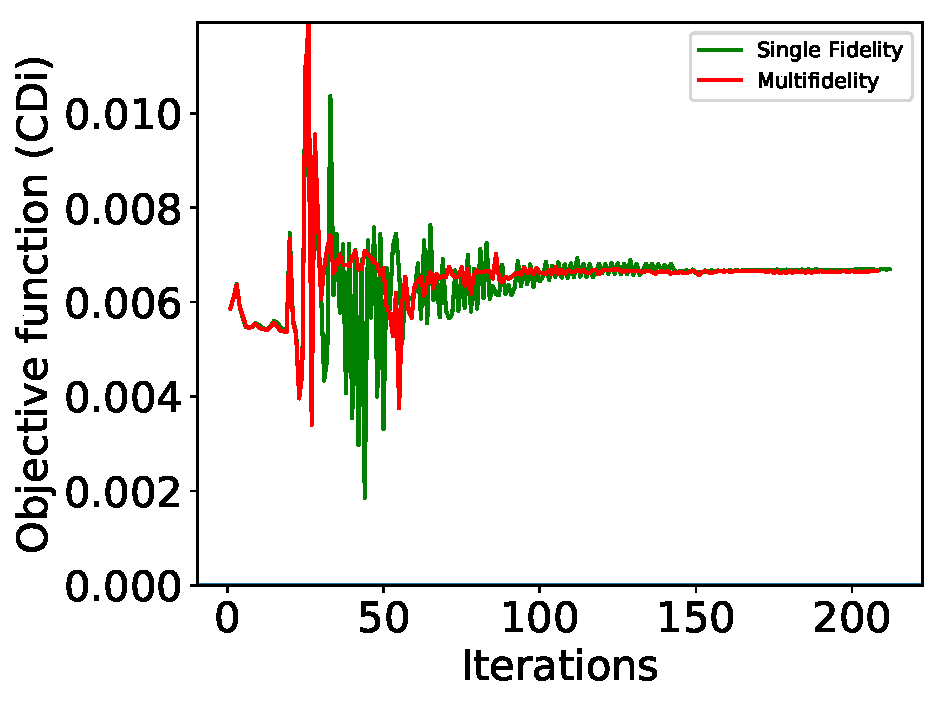
\includegraphics[width=0.9\columnwidth]{images/comparison_objective_sellar.pdf}} \\
\subfloat[Lift Constraint]{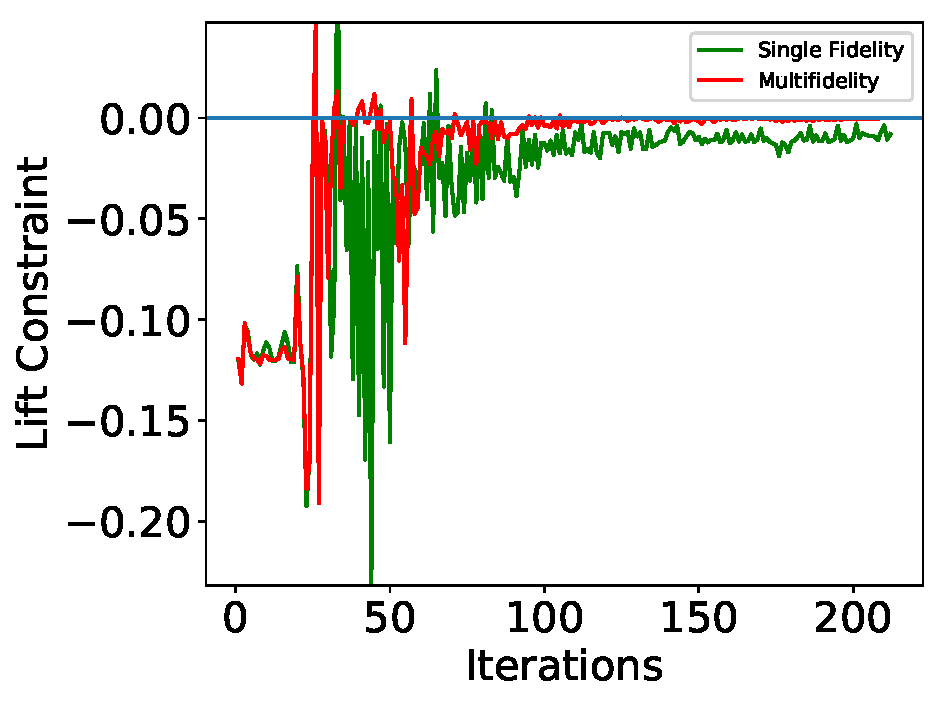
\includegraphics[width = 0.9\columnwidth]{images/mdao_comparison_constraint_1.pdf}} \\
\subfloat[Stress Constraint]{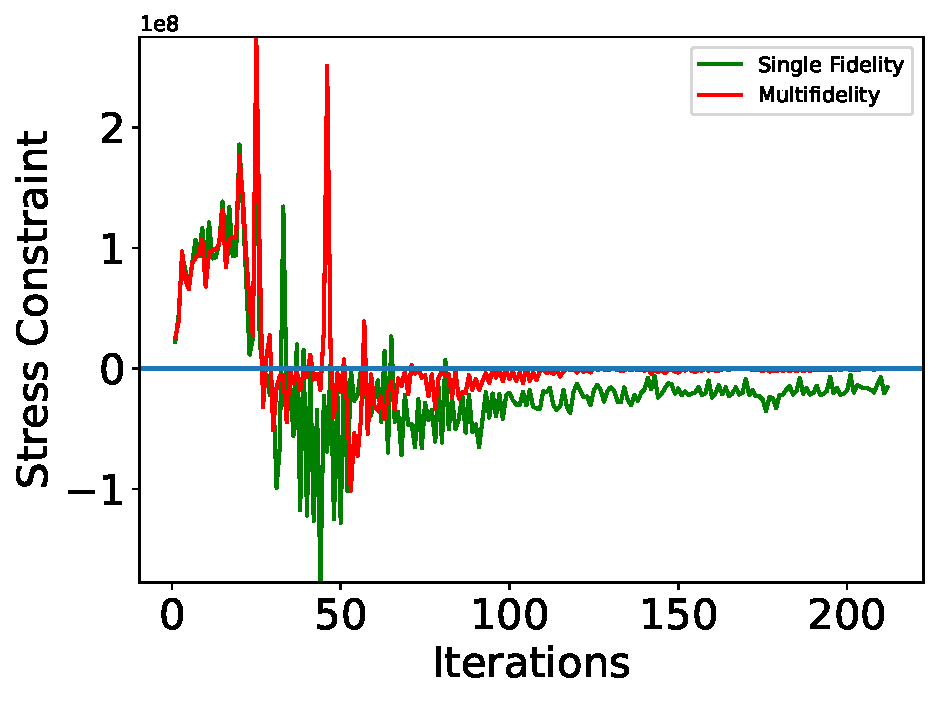
\includegraphics[width = 0.9\columnwidth]{images/mdao_comparison_constraint_2.pdf}} 
\end{tabular}
\caption{Evolution of the solution parameters for both fidelity levels, NASA CRM wing, Panair--Panair}
\label{fig:CRM_sol}
\end{figure}

Fig. \ref{fig:CRM_sol} shows the evolution of the main solution parameters for this case in both single and multifidelity modes. When it comes to the objective function, it is clear that the amount of iterations to converge is only slightly reduced. On the other hand, both constraints are closer to zero for the multifidelity case. A clear gap between the compared strategies means that constraint compliance is never as good in single fidelity mode. Which means that for the same solution, one could reduce the optimizer iterations and get to a similar overall configuration that satisfies the imposed constraints just as well. 
An implementation using ADFlow as the high fidelity fluid solver was explored as well. However, despite the numerous attempts, the solution of the problem never converged. This was due to the fact that the partial solutions from the low fidelity MDA contained regions with geometries that caused the CFD solution to diverge. Since the CFD mesh could not be manually corrected at each step, ADFlow crashed at a certain point and thus the optimizer as well.

\subsection{Blended Wing Body}
In this case, the optimization variable to minimize is the fuel consumption (calculated using the Breguet equation). The parameters and baseline geometry are available in the tutorial section of the \href{https://github.com/mid2SUPAERO/RP_MAE_GILBERTO_RUIZ_JIMENEZ}{GitHub repository}. Fig. \ref{fig:BWB_sol} shows the structural and aerodynamic solution at the end of the optimization loop for the single fidelity case. After successfully solving the problem in single fidelity, the aerodynamic mesh was refined using a python library developed at ONERA: CASIOPÉE \cite{Benoit2015}. 

\begin{figure}[htpb]
\centering
\begin{tabular}{c}
\subfloat[Cp distribution]{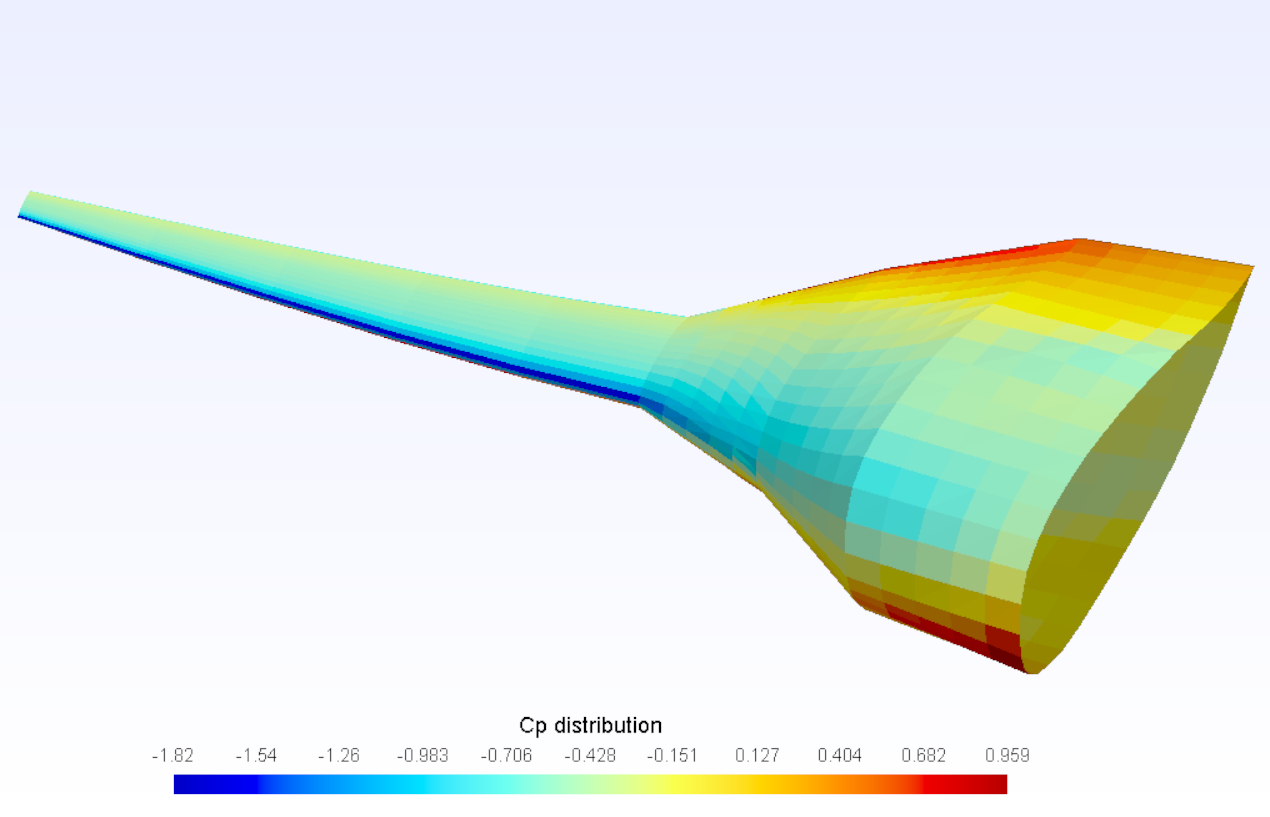
\includegraphics[width=0.9\columnwidth]{images/BWB_cp_dist.PNG}} \\
\subfloat[Equivalent Von Mises Stress (MPa)]{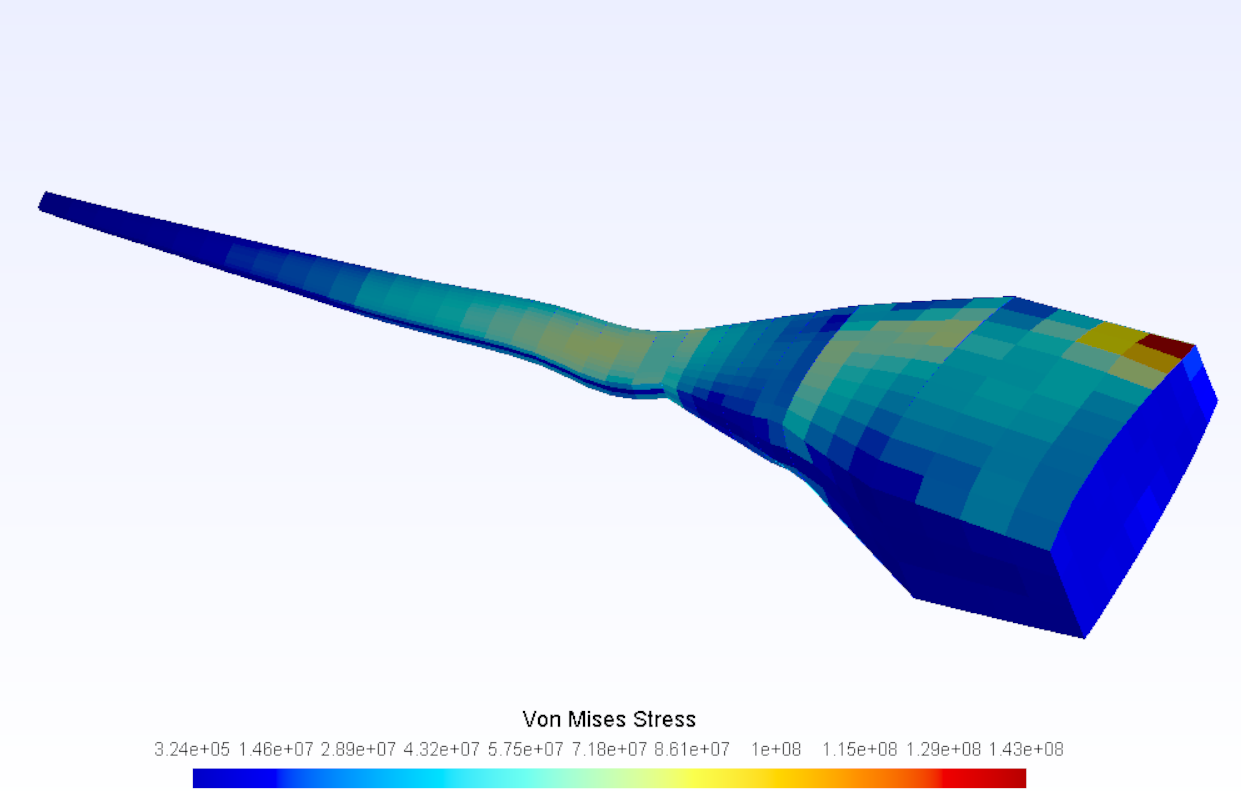
\includegraphics[width = 0.9\columnwidth]{images/BWB_vonmises_dist.PNG}} 
\end{tabular}
\caption{Optimization result for the BWB case, single fidelity.}
\label{fig:BWB_sol}
\end{figure}

A series of issues arose after the mesh refinement for the high fidelity case, mainly that the enriched geometry had some non-convex panels that were not compatible with the high order panel code. As a consequence, the refinement was repeated, this time only doubling the mesh nodes instead of tripling them. In this case, Panair did not crash, but the resulting Cp distribution had some panels with undefined values. This, in turn, causes the optimizer to crash because it cannot parse the current vector into the inner algorithm. Despite numerous attempts to create a viable high-fidelity mesh for Panair, the very well known issue of convexity between panels prevented a smooth run of the current method. \par 
Just like in the previous test case, an implementation using ADFlow as the high fidelity fluid solver was explored. The geometry in is now even more complex, hence, it was not surprising to get the same crash of the program after some optimizer runs, this time due to the large deformations of the structure produced by the optimizer, which in turn generate spikes in the aerodynamic mesh that cause the CFD code to fail.  

\subsection{Analytical functions}
With the aim of validating the performance of the simple transfer strategy, 5 different analytical formulations of a high and low fidelity functions \cite{Bryson2018} were combined with the classic Sellar problem \cite{Sellar1996} and programmed in OpenMDAO along with the filter component to transfer data from the low fidelity MDA to the high fidelity MDA. The problems include an expensive function and a close cheap approximation that lacks local details. As described in \cite{Bryson2018}:
\begin{quoting}
Two high fidelity functions (Rosenbrock and Brown) have single minima, while the others are multimodal. The test suite encompasses a variety of mathematical forms, including polynomials, sinusoids, and exponentials.
\end{quoting} All of the formulations are listed in the Appendix A, alongside with the corresponding plots of the results. The sample problems were solved using two different optimization algorithms: COBYLA and SLSQP. Tab. \ref{tab:Analytical} summarizes the results of the tests. 
\par As usual, the efficiency of the optimization algorithm depends heavily on the local characteristics of the objective functions. The present strategy works best with the Styblinski-Tang formulation, and its worst performance occurs with the Rosenbrock function. This tendency was maintained for both optimizer strategies, which confirms that it is the shape of the functions and not the optimizer what makes a problem more suitable for acceleration with the current strategy. A marked difference in the amount of optimization between SLSQP and COBYLA is observed, this is expected because of the advantage of a defined gradient function in the case of SLSQP and has nothing to do with the multifidelity strategy.

\begin{table}[htpb]
\caption{Optimizer iterations needed to converge to a minimum, various formulations.}
\resizebox{\columnwidth}{!}{%
\begin{tabular}{l|r|r|r|r|}
\cline{2-5}
 & \multicolumn{2}{c|}{\textbf{COBYLA Iterations}} & \multicolumn{2}{c|}{\textbf{SLSQP Iterations}} \\ \hline
\multicolumn{1}{|l|}{\textbf{Formulation}} & \multicolumn{1}{l|}{Single} & \multicolumn{1}{l|}{Multifidelity} & \multicolumn{1}{l|}{Single} & \multicolumn{1}{l|}{Multifidelity} \\ \hline
\multicolumn{1}{|l|}{McCormick} & 55 & 55 & 11 & 19 \\ \hline
\multicolumn{1}{|l|}{Brown} & 63 & 124 & 13 & 27 \\ \hline
\multicolumn{1}{|l|}{Styblinski-Tang} & 122 & 120 & 17 & 15 \\ \hline
\multicolumn{1}{|l|}{Rosenbrock} & 61 & 164 & 20 & 26 \\ \hline
\multicolumn{1}{|l|}{Trigonometric} & 83 & 172 & 12 & 14 \\ \hline
\end{tabular}%
}
\label{tab:Analytical}
\end{table}

In order to characterize the compatibility of a problem with the current strategy, a simple proportional parameter was proposed and calculated at each fidelity switch in the previous formulations. Matematically, it is defined as: \begin{equation}
    \beta=\frac{y_2(y_{1_{h}})}{y_2(y_{1_{l}})}
\end{equation}
With this computation, the best, intermediate and worst functions were compared. Fig. \ref{fig:betaplots} shows the two corresponding plots of $\beta$ as the solution of the MDAO advances with each fidelity switch. One can see that the coefficient in the case of the Rosenbrock function is very high, reaching values much larger than 1. On the other hand, the Styblinski-Tang beta coefficient is at all times smaller than 1, which would be expected when the predicting capability of the low fidelity function is very good. The McCormick function has values that at most get to 1, which corresponds to the similarity between both strategies (single fidelity and multifidelity). 

\begin{figure}[htpb]
\centering
\begin{tabular}{c}
\subfloat[Rosenbrock (worst) -McCormick (intermidiate)]{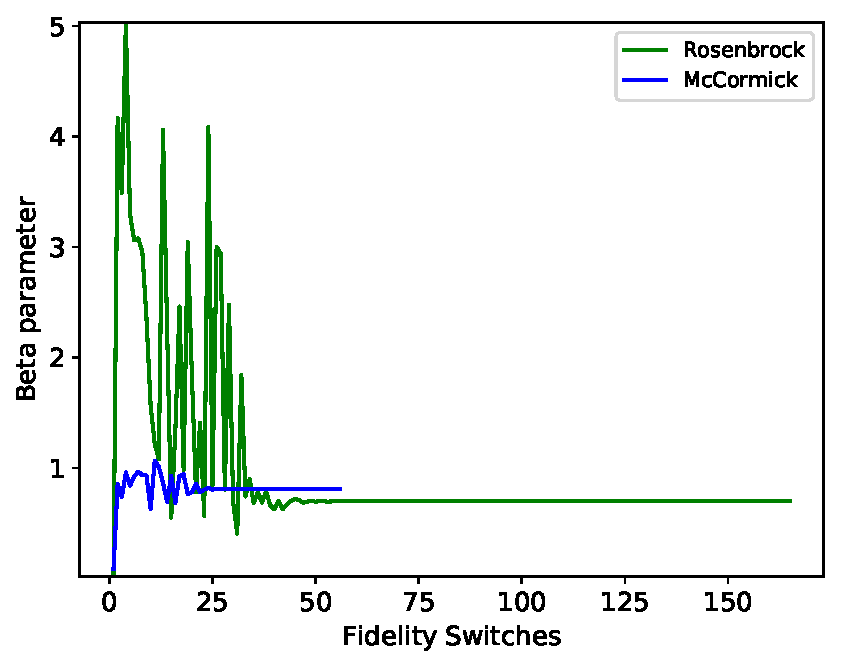
\includegraphics[width=0.9\columnwidth]{images/plot_beta_McCormick_Rosenbrock.pdf}} \\
\subfloat[Styblinski (best) - McCormick (intermidiate)]{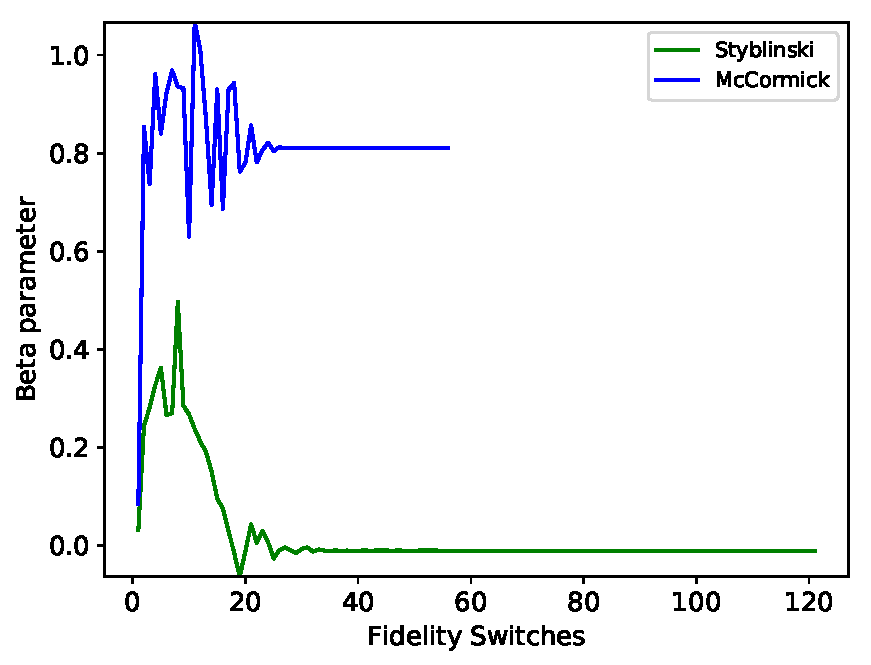
\includegraphics[width = 0.9\columnwidth]{images/plot_beta_McCormick_Styblinski.pdf}} 
\end{tabular}
\caption{Comparison of the beta parameter for the analytical functions with respect to the fidelity switches}
\label{fig:betaplots}
\end{figure}

\section{Conclusions and perspectives}
\label{sec:conclusions}
After a thorough review of different implementations of the presented method, it was shown that the constraint compliance is the main part of the MDAO problem that benefits from the exchange of information between fidelities. The overall number of optimizer calls is only slightly reduced, however, one must remember that the simplicity of implementation is unlike any other existing strategies. This is all contingent of course on the nature of the low and high fidelity functions, as demonstrated in the analytical test section of this work. \par
Another important issue is the morphing of the structure in a way that does not disrupt the aerodynamic mesh to the point that singularities start to show. This is specifically problematic when the high fidelity method is a CFD solver. Constraining the design variables of the structural solver is one of the solutions, however, this must be done carefully so as not to over-constraint the structural optimization in such a way that the mass reduction from the optimization is affected. \par
Some other improvements could be possible with the inclusion of a scaling strategy that used the computed $\beta$ factor at each step to reduce or increase the weight of the low fidelity function with respect to the high fidelity one. Most of the strategies that follow this path use stochastic predictors or surrogates, but if the objective was to try and keep the model as simple as possible, the case can be made for a linear regression at the displacement field transfer. This could potentially allow to keep the constraint convergence acceleration while also reducing the optimization runs.


\section*{Appendix}

\subsection{Formulation and plots of the analytical function tests}
\label{subsec:formulplots}

\subsubsection{McCormick-Sellar problem}
\begin{equation}
    \begin{matrix}
    \textnormal{Minimize} \: x_1^2+z_2+y_1+e^{-y_2} \\
    \textnormal{with respect to} \: z_1,z_2,x_1 \\
    \textnormal{subject to}  \\
    \frac{y_1}{3.16}-1\geq 0  \\
    1-\frac{y_2}{24}\geq 0 \\
    -10\leq z_1 \leq 10 \\
    0\leq z_2 \leq 10 \\
    0\leq x_1 \leq 10 \\
    \\
    \textnormal{Disc. 1:} \: \left\{\begin{matrix} 
     y_{1_h}=\sin{(z_1+z_2)}+(z_1-z_2)^2\\-\frac{3}{2}z_1+\frac{5}{2}z_2-0.2y_2+x_1+1 \\
    \\
    y_{1_l}=(z_1-z_2)^2+2z_1+2z_2\\-0.2y_2+x_1
    \end{matrix} \right. \\
    \\
    \textnormal{Disc. 2:} \:\: y_2=\sqrt{y_1}+z_1+z_2\\
    \end{matrix}
\end{equation}

\begin{figure}[htpb]
\centering
\begin{tabular}{c}
\subfloat[Objective function]{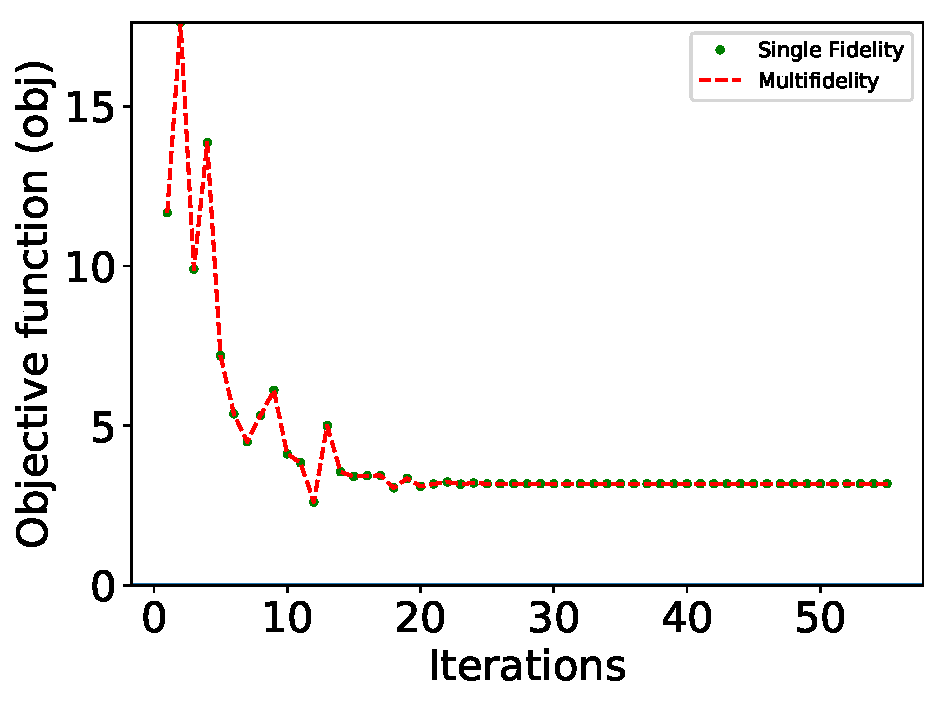
\includegraphics[width=0.4\textwidth]{images/comparison_objective_McCormick.pdf}} \\
\subfloat[Constraint 1]{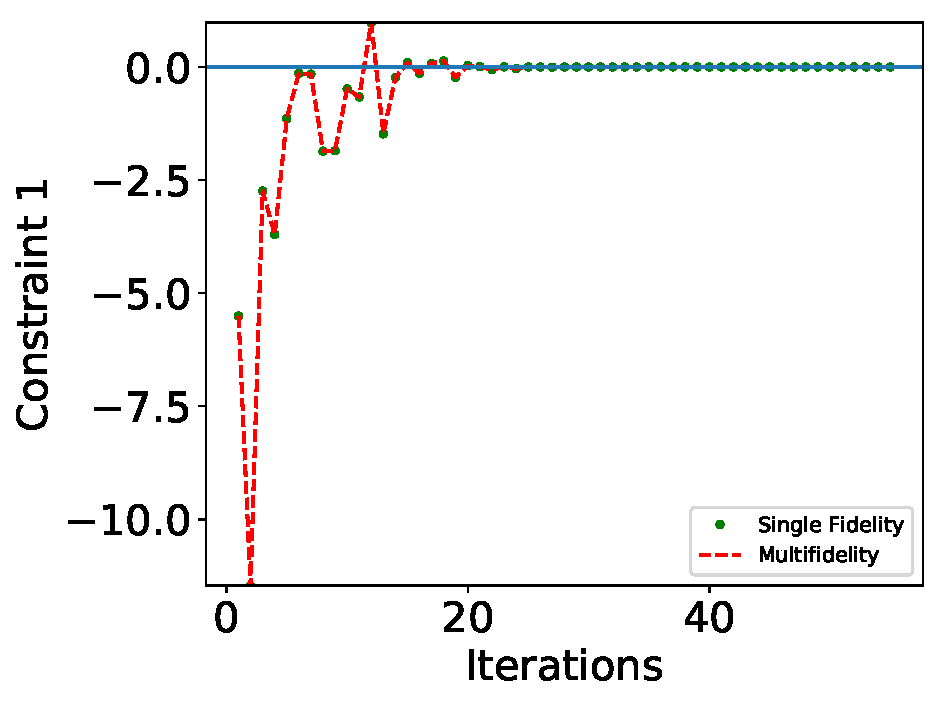
\includegraphics[width = 0.4\textwidth]{images/McCormick_comparison_constraint_1.pdf}} \\
\subfloat[Constraint 2]{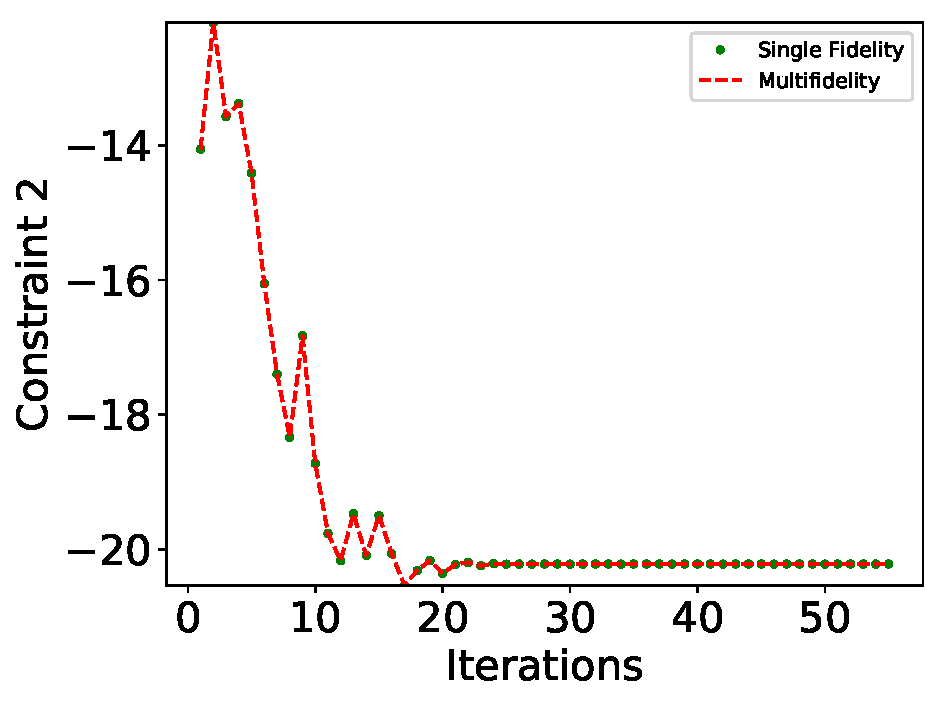
\includegraphics[width = 0.4\textwidth]{images/McCormick_comparison_constraint_2.pdf}} 
\end{tabular}
\caption{Comparison of evolution of solution parameters for the McCormick function}
\label{fig:McCormick_sol}
\end{figure}

\subsubsection{Brown-Sellar problem}
\begin{equation}
    \begin{matrix}
    \textnormal{Minimize} \: x_1^2+z_2+y_1+e^{-y_2} \\
    \textnormal{with respect to} \: z_1,z_2,x_1 \\
    \textnormal{subject to}  \\
    \frac{y_1}{3.16}-1\geq 0  \\
    1-\frac{y_2}{24}\geq 0 \\
    -1\leq z_1 \leq 2 \\
    -1\leq z_2 \leq 2 \\
    0\leq x_1 \leq 10 \\
    \\
    \textnormal{Disc. 1:} \: \left\{\begin{matrix} 
     y_{1_h}=(z_1^2)^{z_2^2+1}+(z_2^2)^{z_1^2+1}+x_1-0.2y_2 \\
    \\
    y_{1_l}=10^{-3}+\exp{(z_1^2+z_2^2)}+x_1-0.2y_2
    \end{matrix} \right. \\
    \\
    \textnormal{Disc. 2:} \:\: y_2=\sqrt{y_1}+z_1+z_2\\
    \end{matrix}
\end{equation}

\begin{figure}[htpb]
\centering
\begin{tabular}{c}
\subfloat[Objective function]{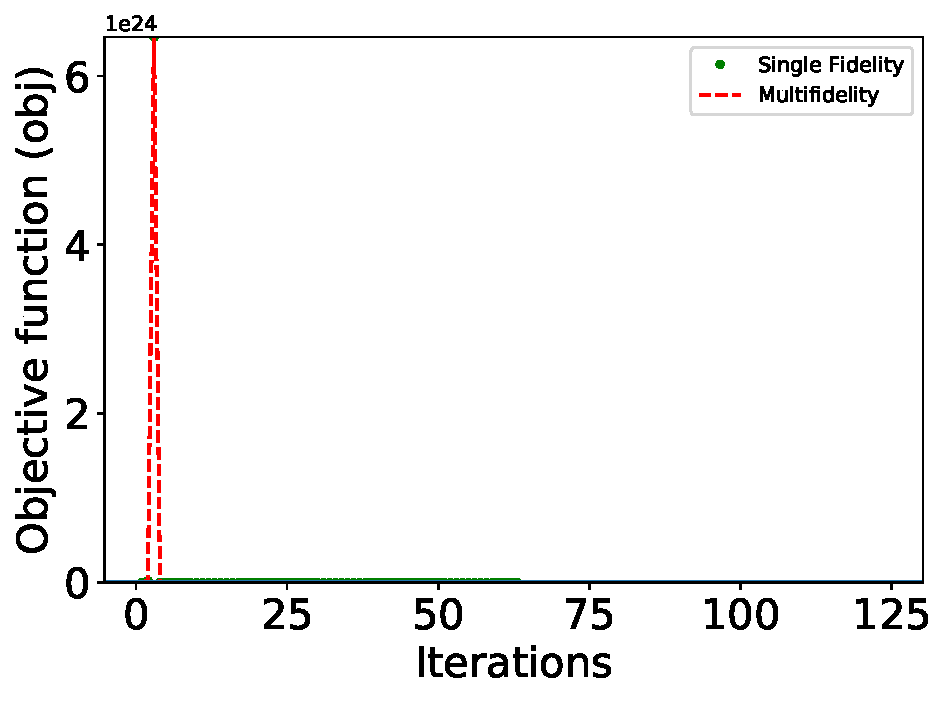
\includegraphics[width=0.4\textwidth]{images/comparison_objective_Brown.pdf}} \\
\subfloat[Constraint 1]{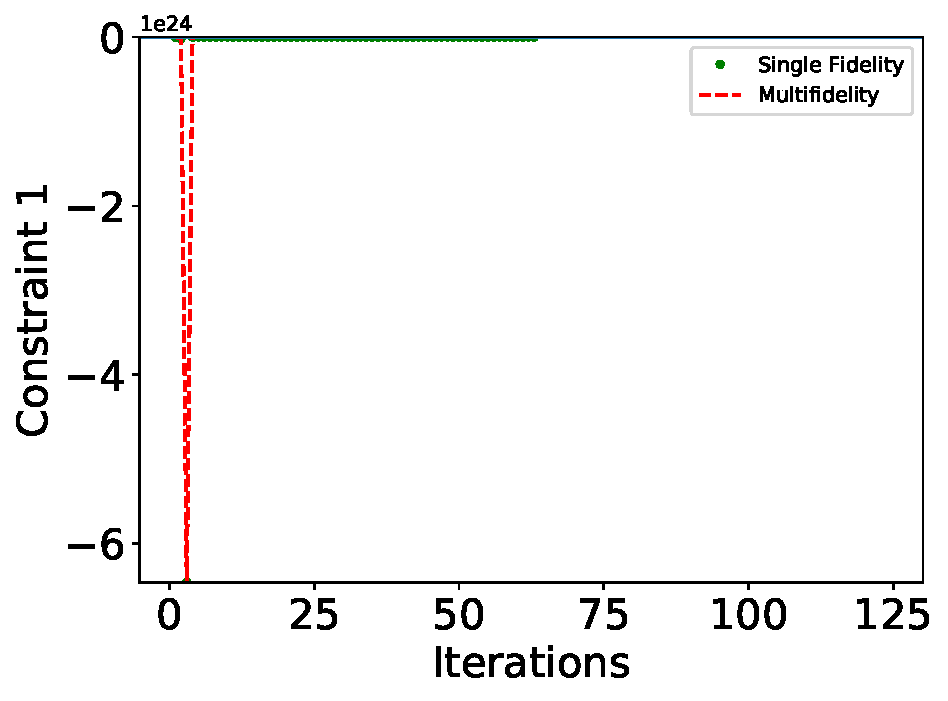
\includegraphics[width = 0.4\textwidth]{images/Brown_comparison_constraint_1.pdf}} \\
\subfloat[Constraint 2]{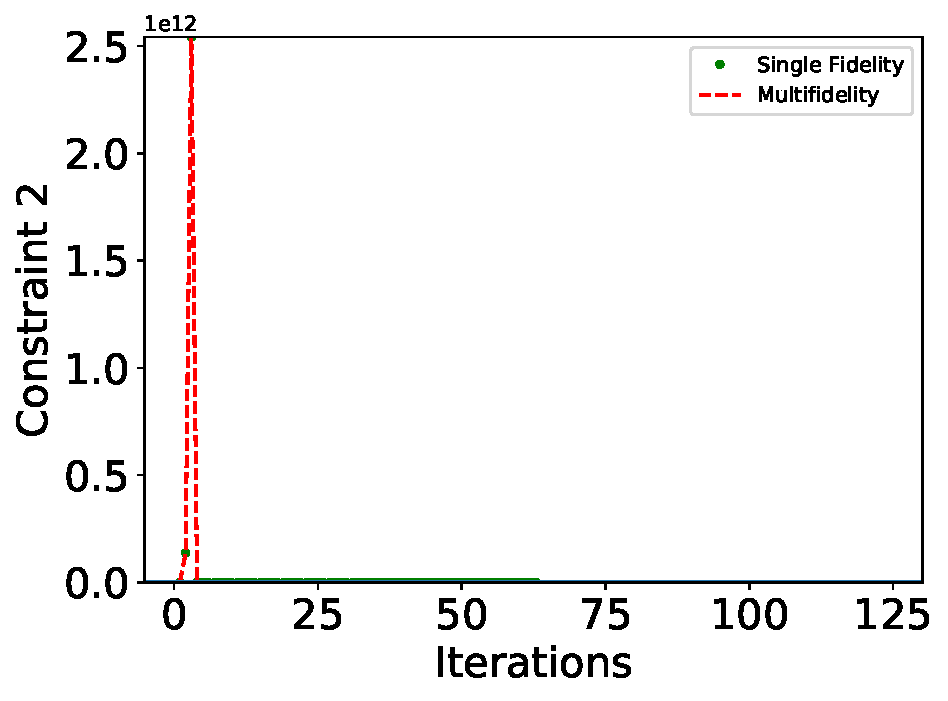
\includegraphics[width = 0.4\textwidth]{images/Brown_comparison_constraint_2.pdf}} 
\end{tabular}
\caption{Comparison of evolution of solution parameters for the Brown function}
\label{fig:Brown_sol}
\end{figure}

\subsubsection{Styblinski-Tang-Sellar problem}
\begin{equation}
    \begin{matrix}
    \textnormal{Minimize} \: x_1^2+z_2+y_1+e^{-y_2} \\
    \textnormal{with respect to} \: z_1,z_2,x_1 \\
    \textnormal{subject to}  \\
    \frac{y_1}{3.16}-1\geq 0  \\
    1-\frac{y_2}{24}\geq 0 \\
    -5\leq z_1 \leq 5 \\
    -5\leq z_2 \leq 5 \\
    0\leq x_1 \leq 10 \\
    \\
    \textnormal{Disc. 1:} \: \left\{\begin{matrix} 
     y_{1_h}=\frac{1}{2}\left[\left(z_1^4-16z_1^2+5z_1\right) \right. \\ \left.+\left(z_2^4-16z_2^2+5z_2 \right) \right]+x_1-0.2y_2 \\
    \\
    y_{1_l}=z_1^4\cos\left(\frac{2\pi z_1}{5}\right)+z_2^4\cos\left(\frac{2\pi z_2}{5}\right)\\ +x_1-0.2y_2
    \end{matrix} \right. \\
    \\
    \textnormal{Disc. 2:} \:\: y_2=\sqrt{y_1}+z_1+z_2\\
    \end{matrix}
\end{equation}

\begin{figure}[htpb]
\centering
\begin{tabular}{c}
\subfloat[Objective function]{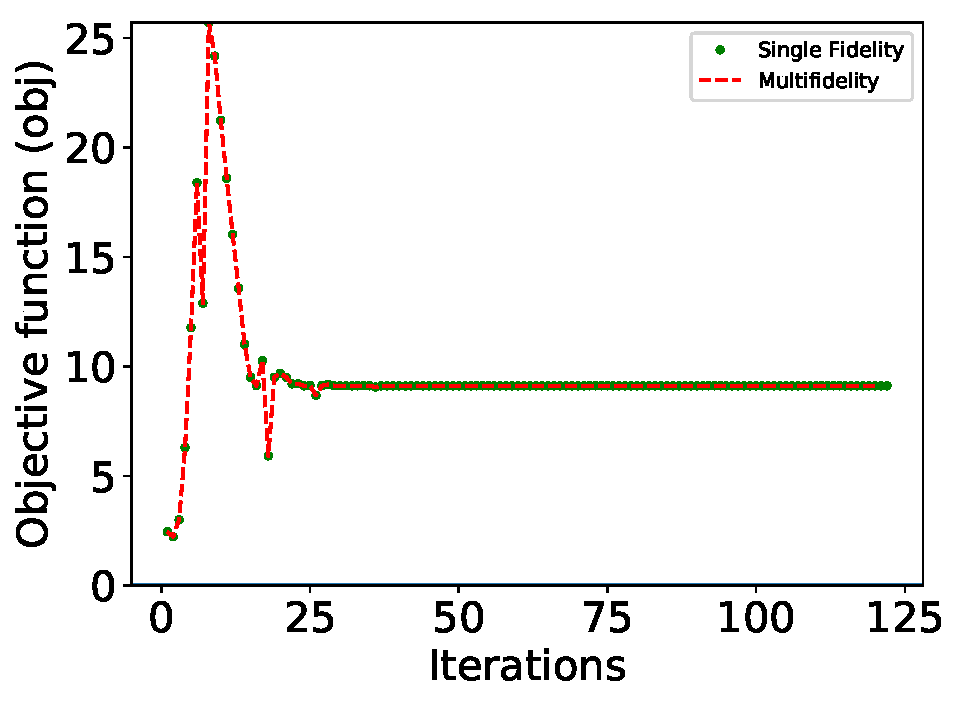
\includegraphics[width=0.4\textwidth]{images/comparison_objective_Styblinski.pdf}} \\
\subfloat[Constraint 1]{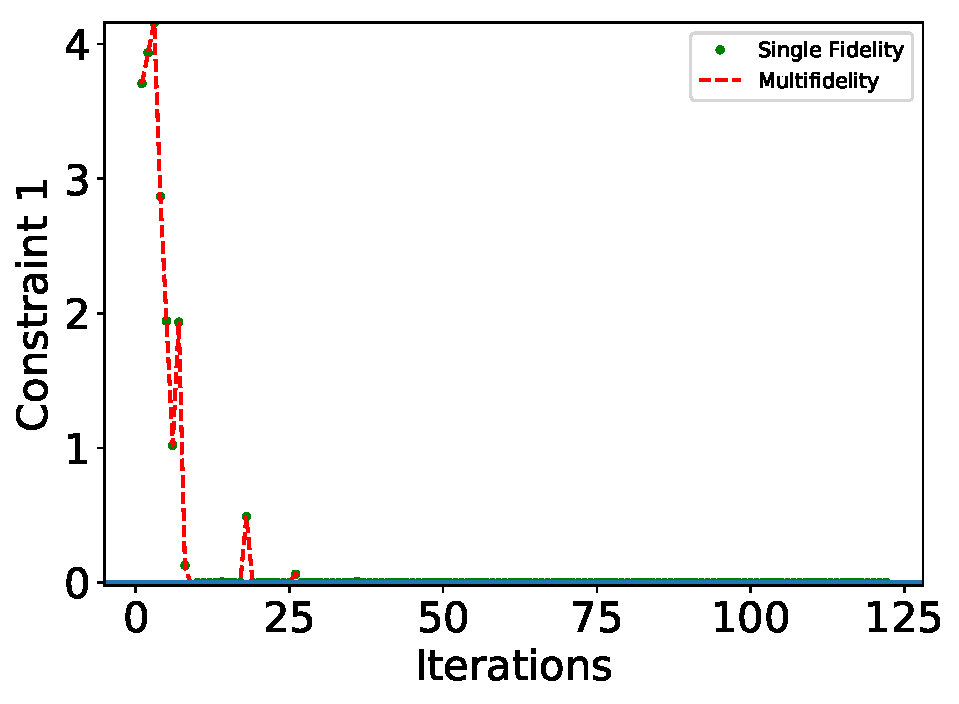
\includegraphics[width = 0.4\textwidth]{images/Styblinski_comparison_constraint_1.pdf}} \\
\subfloat[Constraint 2]{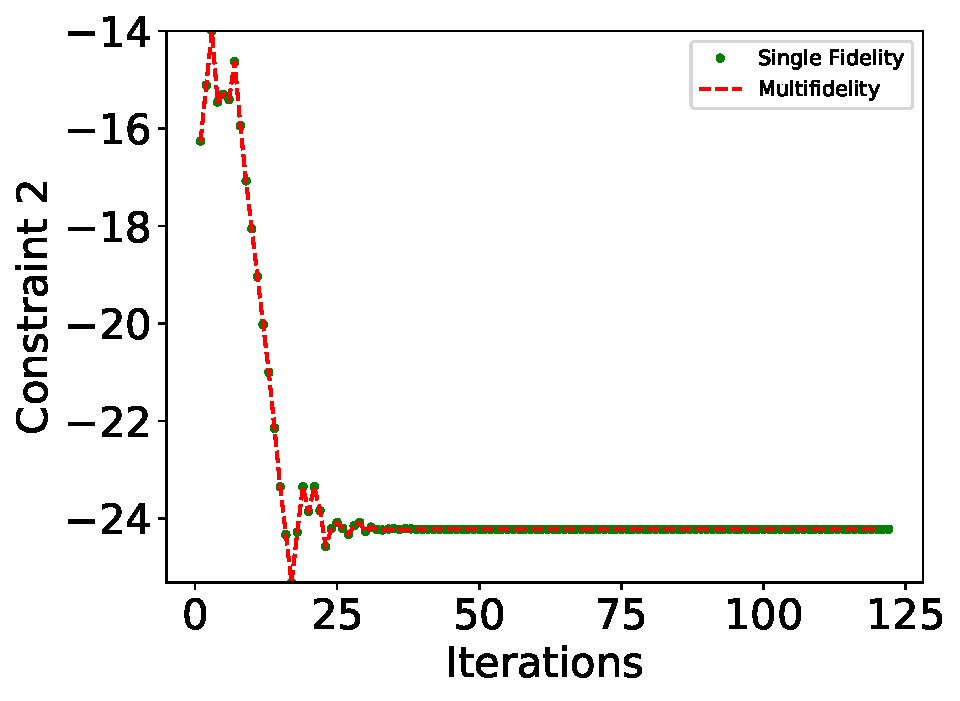
\includegraphics[width = 0.4\textwidth]{images/Styblinski_comparison_constraint_2.pdf}} 
\end{tabular}
\caption{Comparison of evolution of solution parameters for the Styblinski-Tang function}
\label{fig:Styblinski_sol}
\end{figure}

\subsubsection{Rosenbrock-Sellar problem}
\begin{equation}
    \begin{matrix}
    \textnormal{Minimize} \: x_1^2+z_2+y_1+e^{-y_2} \\
    \textnormal{with respect to} \: z_1,z_2,x_1 \\
    \textnormal{subject to}  \\
    \frac{y_1}{3.16}-1\geq 0  \\
    1-\frac{y_2}{24}\geq 0 \\
    -2\leq z_1 \leq 2 \\
    -2\leq z_2 \leq 2 \\
    0\leq x_1 \leq 10 \\
    \\
    \textnormal{Disc. 1:} \: \left\{\begin{matrix} 
     y_{1_h}=(1-z_1)^2+100\left(z_2-z_1^2\right)^2\\+x_1-0.2y_2 \\
    \\
    y_{1_l}=1+50z_1^2\left[(z_2-2)^2+2\right]\\+x_1-0.2y_2
    \end{matrix} \right. \\
    \\
    \textnormal{Disc. 2:} \:\: y_2=\sqrt{y_1}+z_1+z_2\\
    \end{matrix}
\end{equation}

\begin{figure}[htpb]
\centering
\begin{tabular}{c}
\subfloat[Objective function]{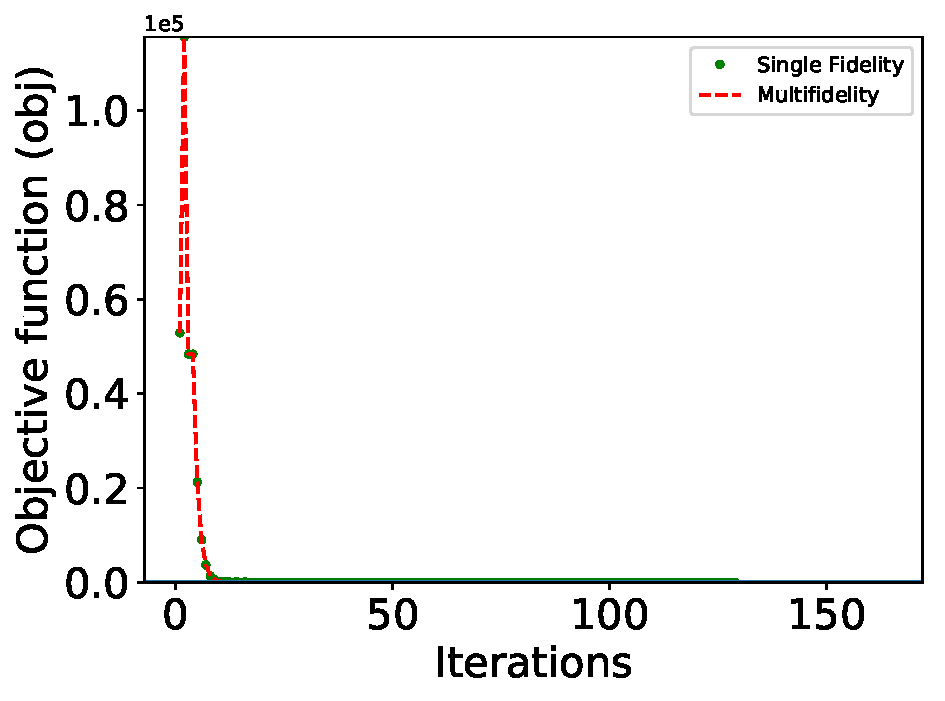
\includegraphics[width=0.4\textwidth]{images/comparison_objective_Rosenbrock.pdf}} \\
\subfloat[Constraint 1]{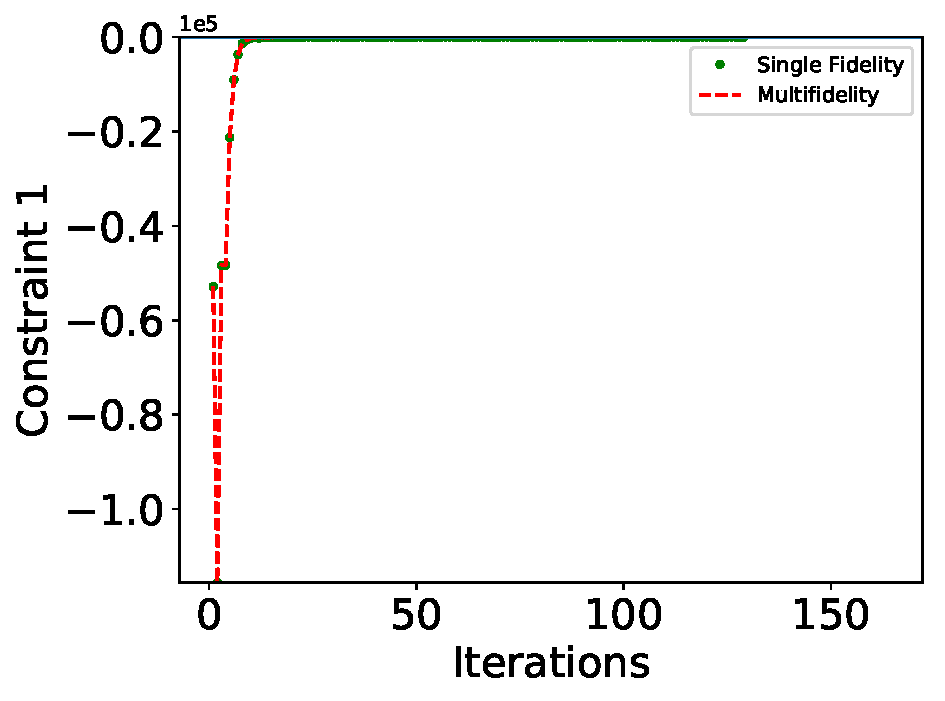
\includegraphics[width = 0.4\textwidth]{images/Rosenbrock_comparison_constraint_1.pdf}} \\
\subfloat[Constraint 2]{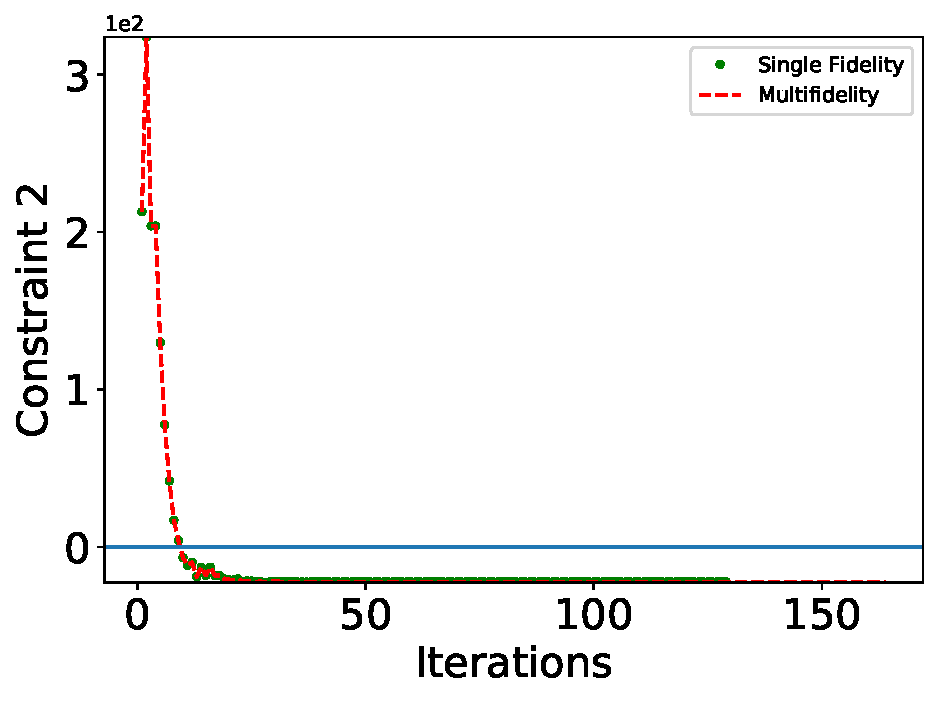
\includegraphics[width = 0.4\textwidth]{images/Rosenbrock_comparison_constraint_2.pdf}} 
\end{tabular}
\caption{Comparison of evolution of solution parameters for the Rosenbrock function}
\label{fig:Rosenbrock_sol}
\end{figure}

\subsubsection{Trigonometric-Sellar problem}
\begin{equation}
    \begin{matrix}
    \textnormal{Minimize} \: x_1^2+z_2+y_1+e^{-y_2} \\
    \textnormal{with respect to} \: z_1,z_2,x_1 \\
    \textnormal{subject to}  \\
    \frac{y_1}{3.16}-1\geq 0  \\
    1-\frac{y_2}{24}\geq 0 \\
    -1.5\leq z_1 \leq 3 \\
    -1.5\leq z_2 \leq 3 \\
    0\leq x_1 \leq 10 \\
    \\
    \textnormal{Disc. 1:} \: \left\{\begin{matrix} 
     y_{1_h}=\sum_{i=1}^{2}\left[2-\sum_{j=1}^{2}\cos(x_j) \right. \\ \left. +i(1-\cos(x_i)-\sin(x_i))\right]^2 \\
    \\
    y_{1_l}=10^{-3}+\sum_{i=1}^{2} 5\left(x_i-\frac{1}{4}\right)\\-0.2y_2+x_1
    \end{matrix} \right. \\
    \\
    \textnormal{Disc. 2:} \:\: y_2=\sqrt{y_1}+z_1+z_2\\
    \end{matrix}
\end{equation}

\begin{figure}[htpb]
\centering
\begin{tabular}{c}
\subfloat[Objective function]{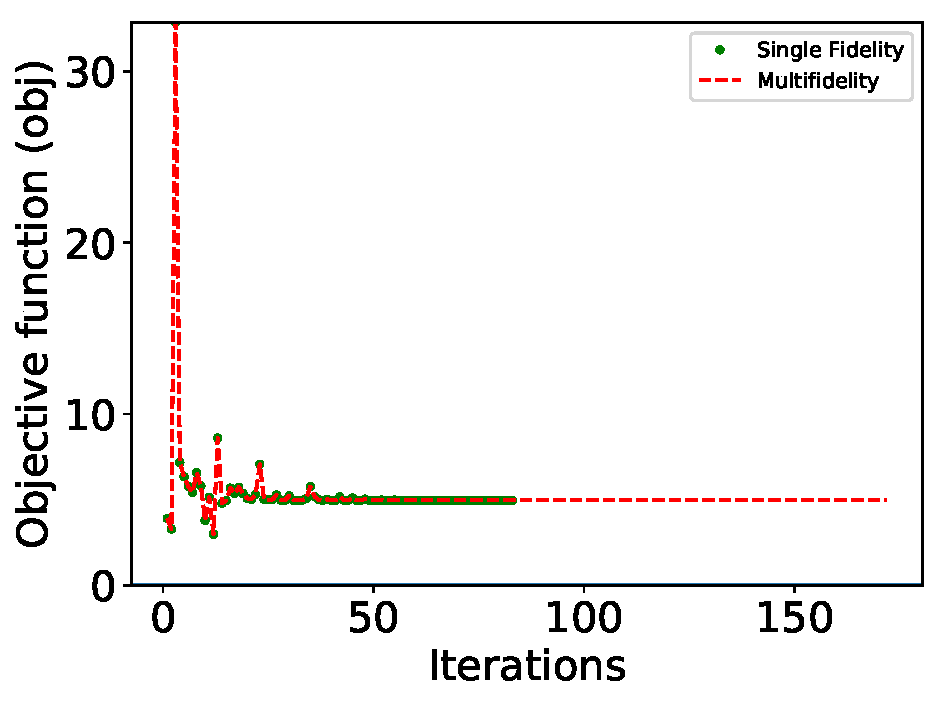
\includegraphics[width=0.4\textwidth]{images/comparison_objective_Trigonometric.pdf}} \\
\subfloat[Constraint 1]{\includegraphics[width = 0.4\textwidth]{images/Trigonometric_comparison_constraint_1.pdf}} \\
\subfloat[Constraint 2]{\includegraphics[width = 0.4\textwidth]{images/Trigonometric_comparison_constraint_2.pdf}} 
\end{tabular}
\caption{Comparison of evolution of solution parameters for the Trigonometric function}
\label{fig:Trigonometric_sol}
\end{figure}

\section*{Acknowledgments}
This work was supported by CONACYT (The Mexican National Council for Science and Technology), grant number 2018-000041-01EXTF-00038.

\bibliography{RPreferences}
\twocolumn[
\begin{@twocolumnfalse}
\section*{Declaration of Authenticity}
This assignment is entirely my own work. Quotations from literature are properly indicated with appropriated references in the text. All literature used in this piece of work is indicated in the bibliography placed at the end. I confirm that no sources have been used other than those stated. \par 
I understand that plagiarism (copy without mentioning the reference) is a serious examinations offence that may result in disciplinary action being taken.
\\
\\
\\
\\

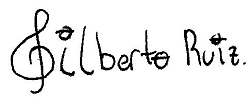
\includegraphics[width=0.35\textwidth, center]{images/Firma.png}\vspace{-0.8cm}
\today \hspace{6 pt} Signature: \hrulefill

\hspace*{0mm}\phantom{\today  Signature: }Gilberto RUIZ JIMÉNEZ, B.Eng.

\hspace*{0mm}\phantom{\today  Signature: }M.Sc. in Aerospace Engineering Student

\end{@twocolumnfalse}
]

\end{document}
